近年、様々なビデオ会議アプリケーション(図\ref{fig:1})が登場している。
その例としては、zoom\cite{1}やGoogle Meet\cite{2}が挙げられる。
新型コロナウイルス感染症の流行により、ビデオ会議の需要がさらに高まりつつある。
\begin{figure}[tb]
  \centering
  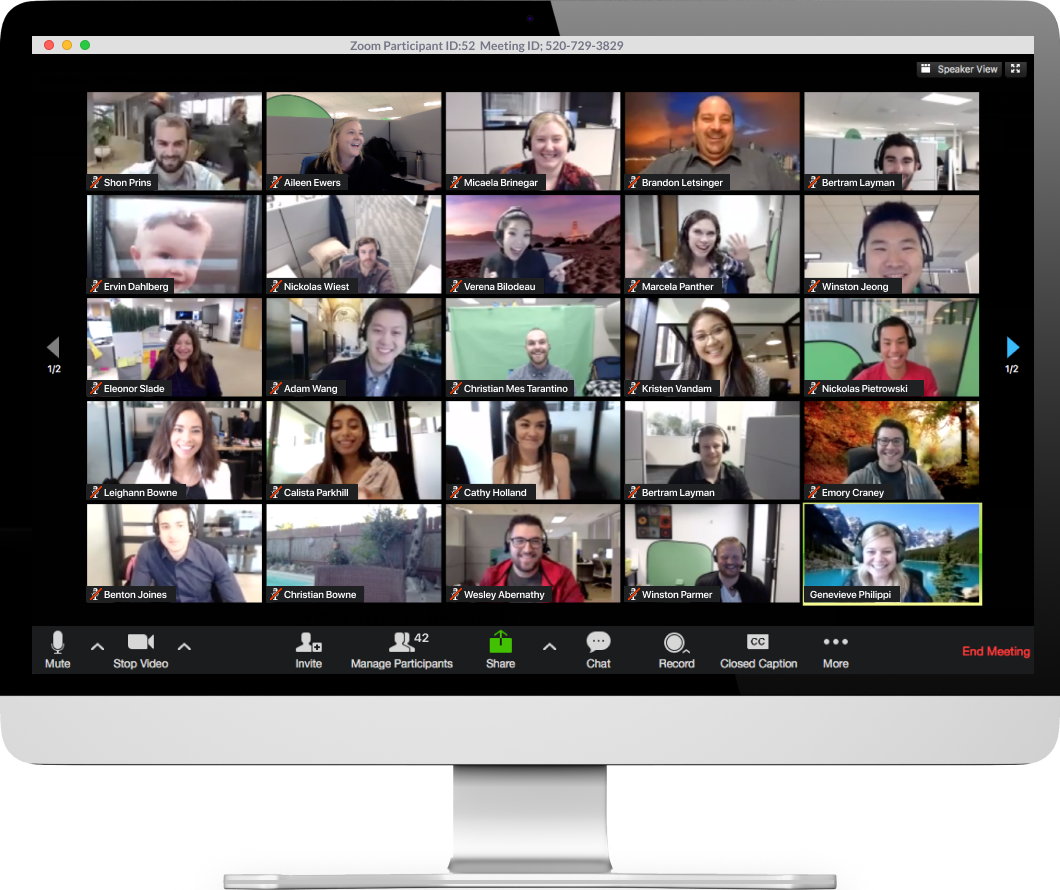
\includegraphics[scale=0.5]{fig/zoom-monitor-screen.png}
  \caption{zoom}\label{fig:1}\cite{1}
\end{figure}

しかし、ビデオ会議における様々な問題点も指摘されている。
例えばRoel\cite{3}は、カメラの視覚外の情報や、人物の情報の不足のために、対面時のような
インタラクションを得られないことを指摘している。

一方で、昨今は誰でも気軽に全天球映像(図\ref{fig:2})を撮影することができるようになっている。
その例として、全天球カメラ(360度カメラ,全天周カメラ,全方位カメラなどともいう (図\ref{fig:3}))
を使用して、全天球映像をヘッドマウントディスプレイを用いて観覧したり、パノラマ映像として動画や静止画を
保存することが出来るようになっている。
\begin{figure}[tb]
  \centering
  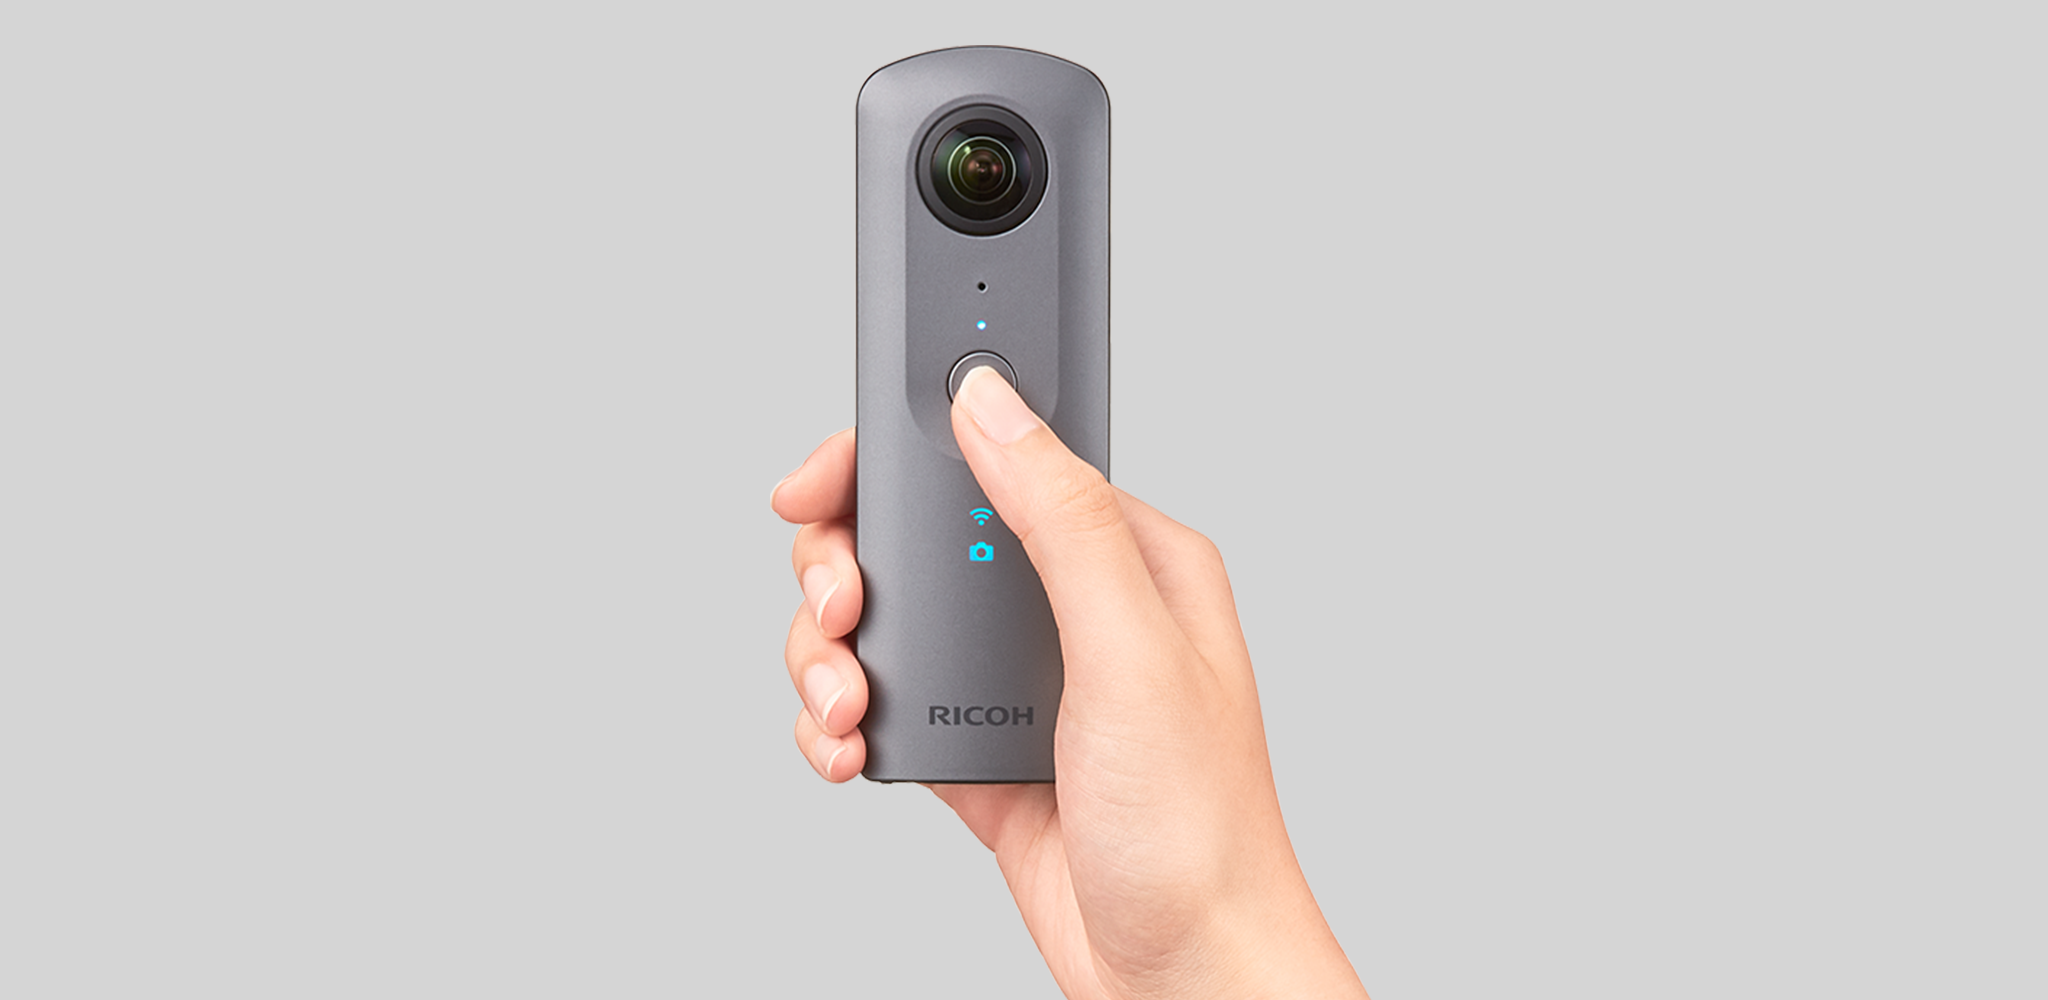
\includegraphics[scale=0.2]{fig/thetaV.png}
  \caption{全天球パノラマ画像}\label{fig:2}
\end{figure}
\begin{figure}[tb]
  \centering
  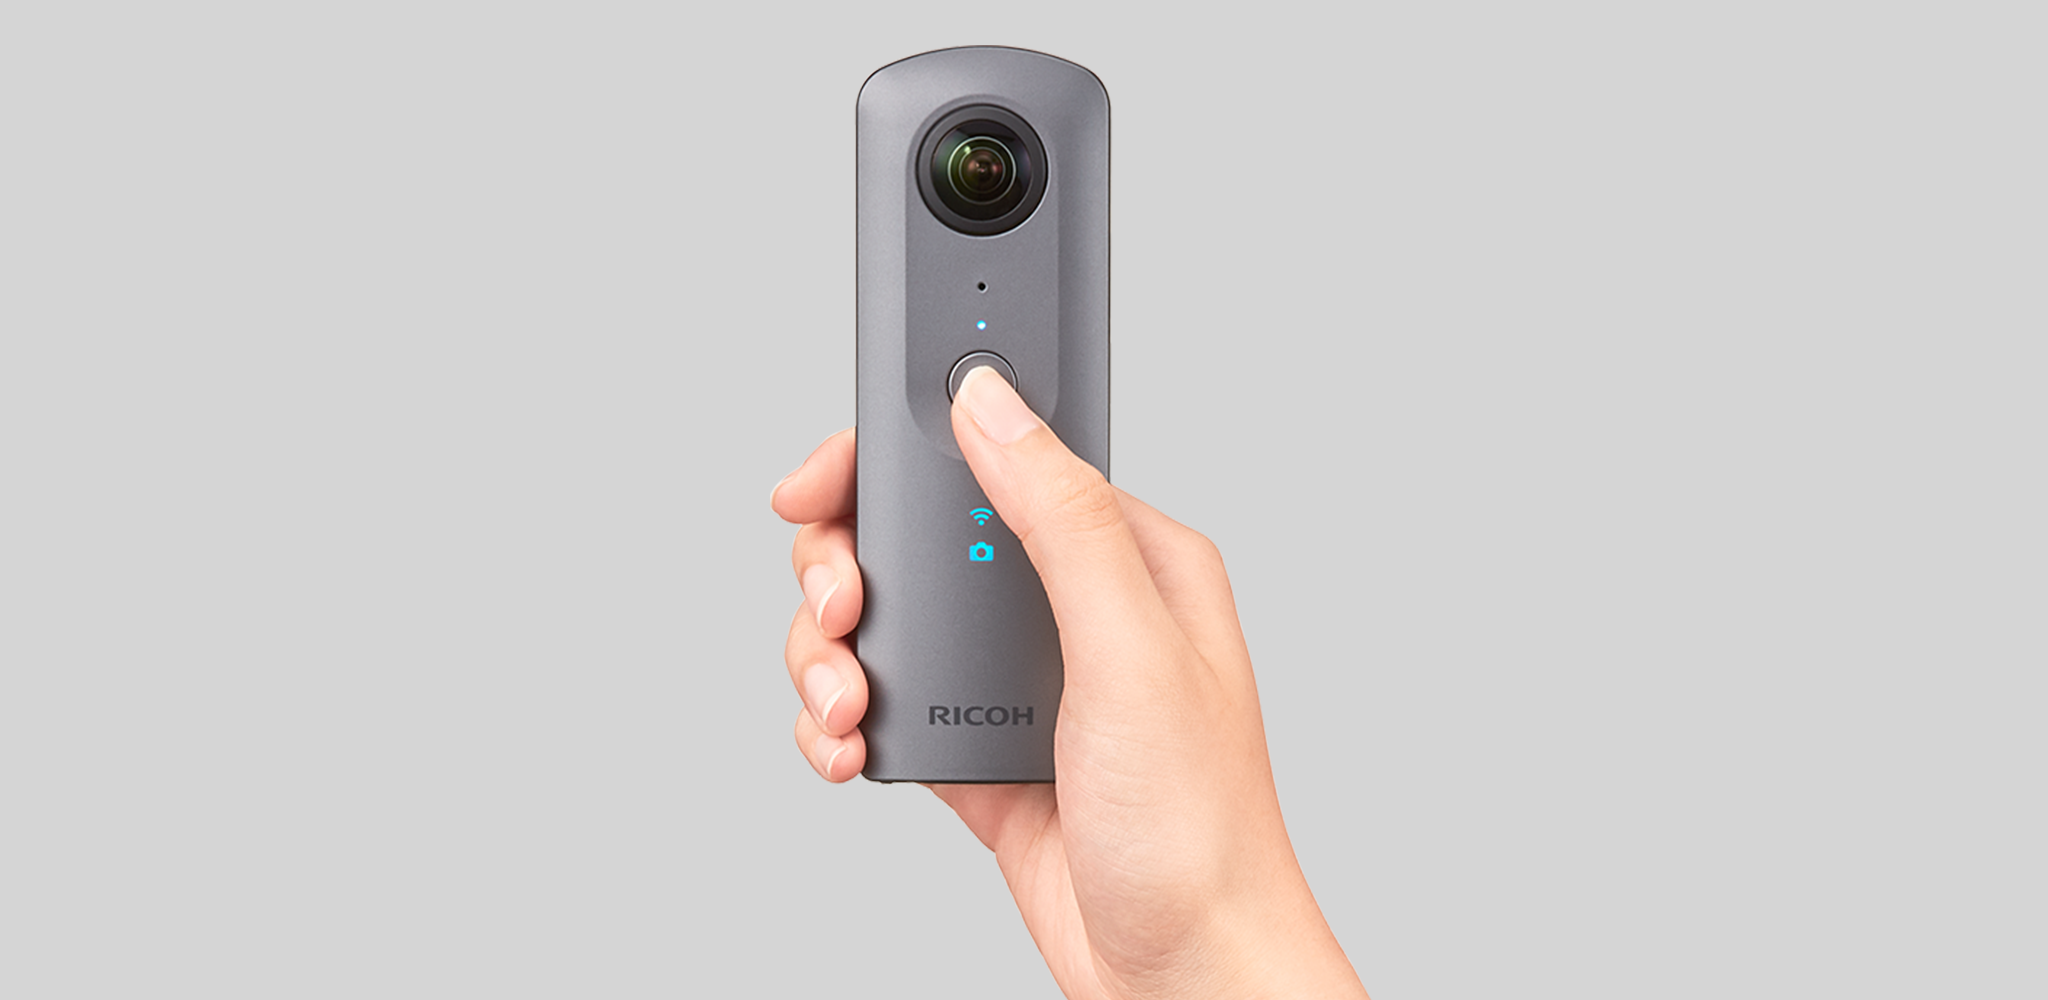
\includegraphics[scale=0.2]{fig/thetaV.png}
  \caption{theta V}\label{fig:3}\cite{4}
\end{figure}

全天周カメラの使用により、カメラの視野の問題は解決される。
実際に、Anthonyら\cite{5}は、全天球の視野の広さによって、リモートユーザーが
ローカルユーザーの環境をより早く理解できると結論付けている。
だが、Johnsonら\cite{6}によって、パノラマ視野によって映像の複雑さが増し、
より大きな認知負荷を必要としたことも示されている。

認知負荷を削減するため、パノラマ映像を3次元に表示する、球体プロジェクターを
用いた方法が挙げられる。球体プロジェクターの利用としては、LiらのOmniEyeBall